\documentclass[a4paper,11pt]{article}
\pagestyle{headings}

\usepackage[utf8]{inputenc}
\usepackage[spanish]{babel}
\usepackage{graphicx}
\usepackage{float}
\usepackage[T1]{fontenc}
\graphicspath{{Documentation/imagenes/}}

\title{Implementación paralela de los algoritmos de "shortest-path" en grafo}
\author{DULERY Romain}
\date{\today}

\setlength{\oddsidemargin}{0.2cm}
\setlength{\evensidemargin}{-0.7cm}
\setlength{\parindent}{30pt}
\setlength{\textwidth}{15cm}
\setlength{\textheight}{24cm}
\setlength{\topmargin}{-.5in}
\setlength{\parskip}{1ex}

\begin{document}

\maketitle
\vspace{1cm}

\section{Presentación general del proyecto y del trabajo realisado}

El proyecto consiste en la implementación paralela de los algoritmos de "shortest-path", en particular los algoritmos de Floyd-Warshall y de Dijsktra.\\\\
El objectivo es que los algoritmos sean utilizados sobre las placas Xeon Phi 3120P, que utilizan openMP con el compilador icc de intel.\\\\
Las technologias usadas fueron C++, OpenMP para paralelizar, y Python3 para hacer scripts. Tambien usé Valgrind para las analisas de desempeño.\\\\
Me concentré en la optimisación del algoritmo de Floyd-Warshall, haciendo muchas versiones diferentes de este algoritmo.\\\\
Hice una plataforma de test de desempeño, para generar automaticamente las matriz de entrada, y los resultados de desempeño para cada algoritmo.\\\\
En la parte siguiente se puede encontrar las metodas usadas en este plataforma, y despues sigue la presentación de los algoritmos realisados.\\\\

\section{Presentación de la plataforma de desarrollo}

Se presenta con la siguiente organización :

\begin{figure}
\begin{center}
  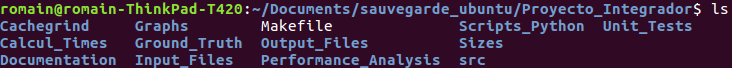
\includegraphics[scale=0.6]{arborescence.png}
  \caption{Organización de la carpeta}
\end{center}
\end{figure}

\subsection{Datos de entrada}

Empezamos con los datos de entrada, que estan en la carpeta llamada Input\_Files.

\subsubsection{Formato de datos}

El formato elegido es el siguiente :

La primera linea indiqua el numero de vértices y de aristas.
Despues cada linea representa una arista, con el numero de vértice de inicio, el numero de vértice de fin, y el peso.

Los numeros de vertices siempre empezan de 0.\\

\noindent Por ejemplo, este grafo :

\begin{figure}[h]
\begin{center}
  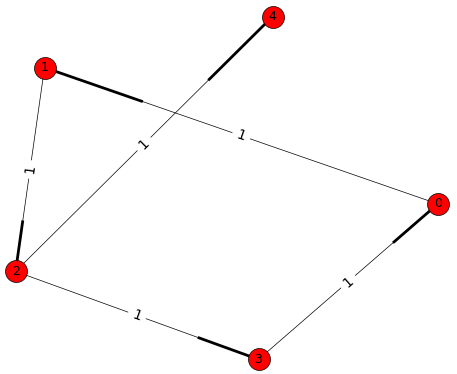
\includegraphics[scale=0.7]{input_exemple.png}
  \caption{Grafo de ejemplo}
\end{center}
\end{figure}

\noindent es representado de la manera siguiente :

\begin{figure}[h]
\begin{center}
  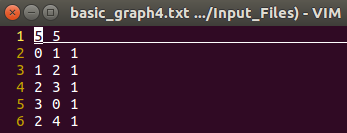
\includegraphics[scale=0.7]{input_graph4.png}
  \caption{Datos de entrada correspondientes}
\end{center}
\end{figure}

\subsubsection{Generación de los archivos de entrada}

En la carpeta Scripts\_Python se pueden encontrar los scripts \textbf{Input\_Files\_Generator.py} y \textbf{Special\_File\_Generator.py} que creen datos de entrada.

El primero genera 30 archivos de entrada con el nombre indicado en argumento 1 y el numero de vertices aleatorio entre V/2 y V, donde V es el numero pasado en argumento 2. Hay tambien el numero de aristas en tercero argumento, aunque no influye la complejidad. El peso de cada arista es aleatorio entre 1 y 100.

El secundo script es lo mismo pero por un solo archivo, con numeros exactos de vertices y aristas.

\subsubsection{Datos utilisados}

\noindent En todo el documento V es el numero de vertices, y E el numero de aristas.

\noindent Usé grafos ordenados en 7 categorias :

\begin{itemize}
  \item basicos (basic\_graphX)\\
    Estan muy simple, sirven para testear el functionamiento basico de los algoritmos.
    El grafo de la Figura 2 es el basic\_graph4.
  \item simples (simple\_graphX)\\
    V entre 5 y 20
    E entre 10 y 30
  \item medios (medium\_graphX)\\
    V entre 100 y 1000
    E entre 200 y 5000
  \item complejos (complex\_graphX)\\
    V entre 1000 y 2000
    E entre 1000 y 10000
  \item re complejos (very\_complex\_graphX)\\
    V entre 2000 y 5000
    E entre 10000 y 50000
  \item enormes (huge\_graphX)\\
    V entre 5000 y 10000
    E entre 50000 y 150000
  \item referencia (reference\_graphX)\\
    Son 6 grafos con V = 400, 800, 1200, 1600, 2000 y 3200
\end{itemize}

\subsection{Datos de salida}

Los datos de salida estan simplemente la matriz de distancias entre cada vertice. Pueden estar salvados en archivos con una opción del main, que esta en la subparte siguiente.

\subsection{Makefile y main}

Al principio hay que generar el main con \textbf{make}. Puede ser usado con \textbf{make debug} o \textbf{make sinopti} para generar el main en version debug o en version sin la optimisación O3 del compilador.

El main pregunta para elegir un archivo de entrada, y despues ejecuta todos los algoritmos con este entrada, monstrando los tiempos de ejecución de cada algoritmo.

\begin{figure}[H]
\begin{center}
  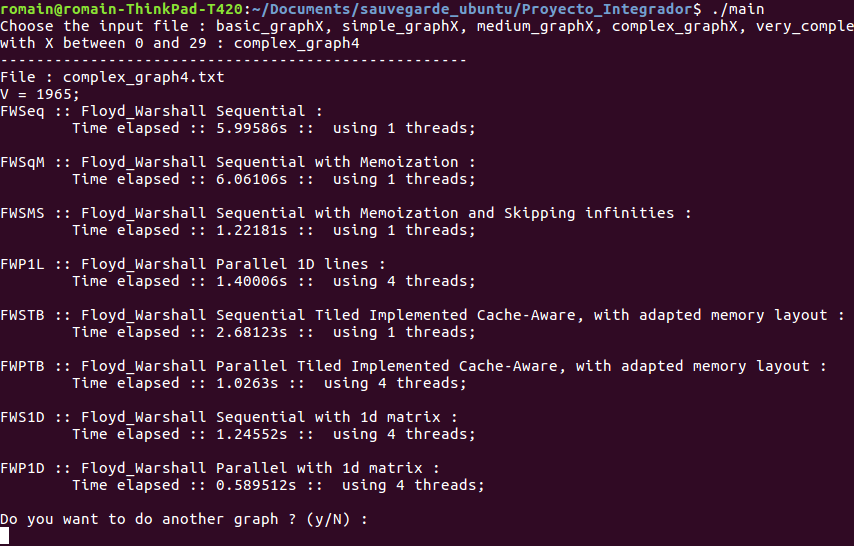
\includegraphics[scale=0.7]{main.png}
  \caption{Una ejecución del main}
\end{center}
\end{figure}

\noindent El main tiene tambien bastante opciones para usarlo de manera diferente, hay :

\begin{itemize}
    \item -a : para elegir un solo algoritmo
    \item -d : para salvar los datos de salida de cada algoritmo en archivos, en la carpeta Output\_Files
    \item -t : para salvar los tiempos de ejecución para cada entrada en archivos, en la carpeta Calcul\_Times
    \item -c : para tomar todas las entradas de una categoria (simple, medios, complejos...)
    \item -g : para elegir el grafo de entrada
    \item -h : para mostrar la ayuda
    \item -s : para elegir el paso de algunos algoritmos que estan presentados en la parte siguiente.
\end{itemize}

\section{Presentacion de cada algoritmo}

Cada algoritmo tiene un codigo de entrada y un codigo de salida.

El codigo de entrada sirve para la opción -a del main, y el codigo de salida sirve para la opción -t del main.

\subsection{Floyd-Warshall secuencial}

\noindent Codigo de entrada : FW\_SEQ \\
Codigo de salida : FWSeq

\begin{figure}[H]
\begin{center}
  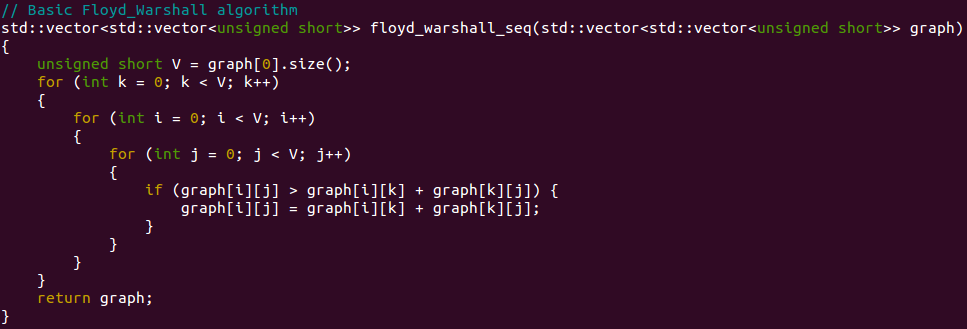
\includegraphics[scale=0.7]{FW_SEQ.png}
  \caption{Algoritmo de Floyd-Warshall}
\end{center}
\end{figure}

Es el algoritmo basico de Floyd-Warshall.

\subsection{Floyd-Warshall secuencial con memoización}

\noindent Codigo de entrada : FW\_SEQ\_MEM \\
Codigo de salida : FWSqM

\begin{figure}[H]
\begin{center}
  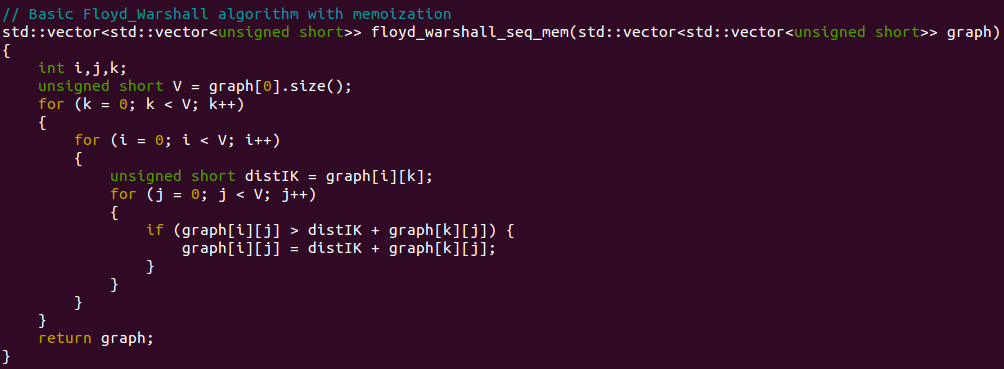
\includegraphics[scale=0.6]{FW_SEQ_MEM.png}
  \caption{Algoritmo de Floyd-Warshall con memoización}
\end{center}
\end{figure}

Es el algoritmo basico, con memorisacion de la distancia IK, porque es recalculada cada vez para nada en la bucle sobre j.

Eso permite tambien de reducir el numero de fallas de cache.

\subsection{Floyd-Warshall secuencial con memoizacion y saltando infinitos}

\noindent Codigo de entrada : FW\_SEQ\_MEM\_SKIP \\
Codigo de salida : FWSMS

\begin{figure}[H]
\begin{center}
  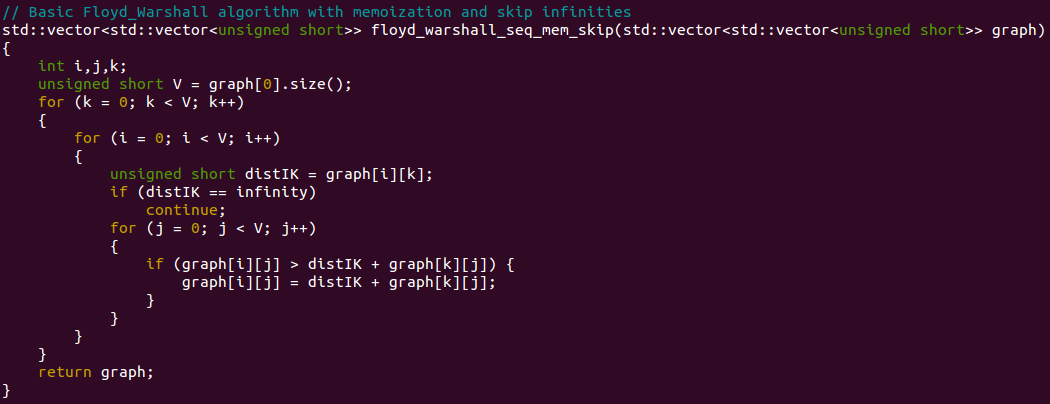
\includegraphics[scale=0.6]{FW_SEQ_MEM_SKIP.png}
  \caption{Algoritmo de Floyd-Warshall con memoización y saltos de infinitos}
\end{center}
\end{figure}

Es el algoritmo basico, con memorisacion de la distancia IK, y saltando las columnas que tienen una valor infinita.

Cada algoritmo que sigue utiliza este memorisacion y salta las valores infinitas.

\subsection{Floyd-Warshall paralelizado sobre las lineas}

\noindent Codigo de entrada : FW\_PAR1\_L \\
Codigo de salida : FWP1L

\begin{figure}[H]
\begin{center}
  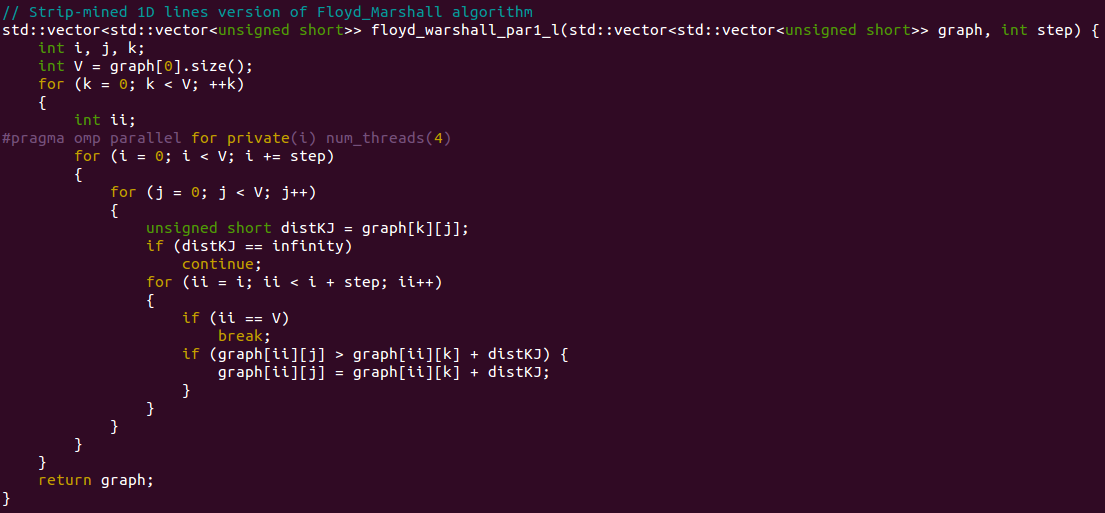
\includegraphics[scale=0.6]{FW_PAR1_L.png}
  \caption{Algoritmo de Floyd-Warshall parelelo sobre las lineas}
\end{center}
\end{figure}

La matriz es cortada en bloques horizontales, y cada thread trabaja sobre un bloque.

\subsection{Floyd-Warshall paralelizado sobre las columnas}

\noindent Codigo de entrada : FW\_PAR1\_C \\
Codigo de salida : FWP1C

\begin{figure}[H]
\begin{center}
  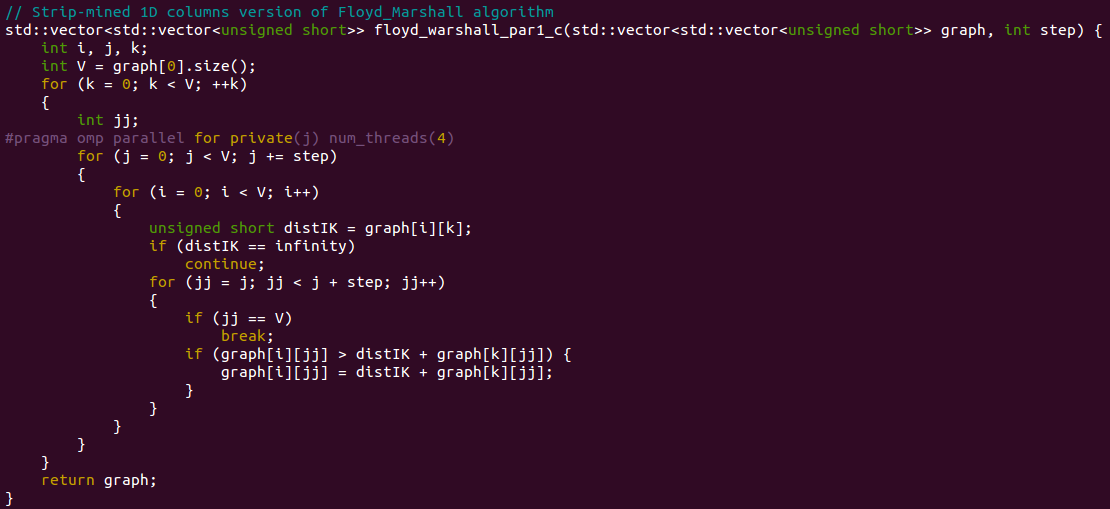
\includegraphics[scale=0.6]{FW_PAR1_C.png}
  \caption{Algoritmo de Floyd-Warshall parelelo sobre las columnas}
\end{center}
\end{figure}

Es lo mismo que el algoritmo de antes, pero sobre las columnas.

\subsection{Floyd-Warshall secuencial, con una matriz cortada en bloques cuadrados}

\noindent Codigo de entrada : FW\_SEQ\_TILED \\
Codigo de salida : FWSTI (Floyd-Warshall sequential tiled-implemented)

\begin{figure}[H]
\begin{center}
  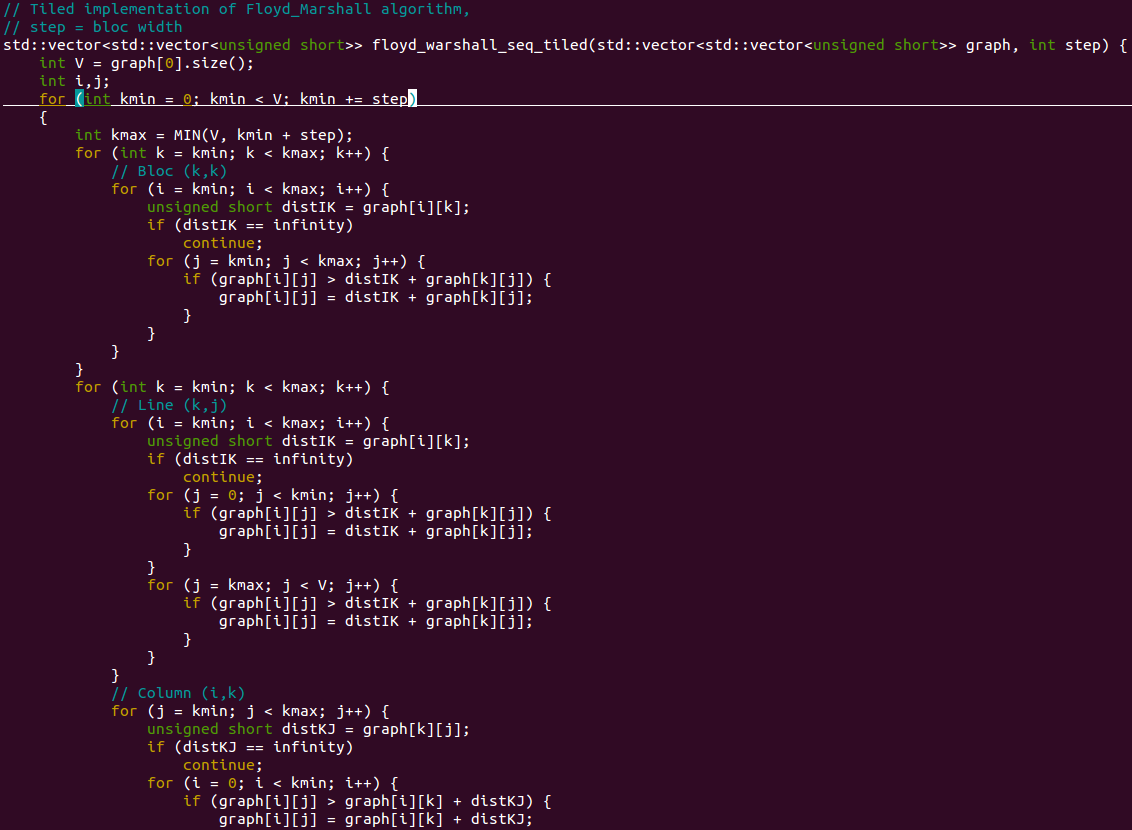
\includegraphics[scale=0.6]{FW_SEQ_TILED.png}
  \caption{Algoritmo de Floyd-Warshall con una matriz cortada en bloques}
\end{center}
\end{figure}

Es un algoritmo de transicion hasta el algoritmo siguiente.

La idea es de cortar la matriz en bloques cuadrados, y de tratarla en un orden particular :

\begin{minipage}{0.50\linewidth}
  \begin{enumerate}
    \item El bloque (k, k)
    \item La linea y la columna del bloque, que solo depienden del bloque (k,k)
    \item Lo que queda
  \end{enumerate}
\end{minipage}\hfill
\begin{minipage}{0.4\linewidth}
  \begin{center}
    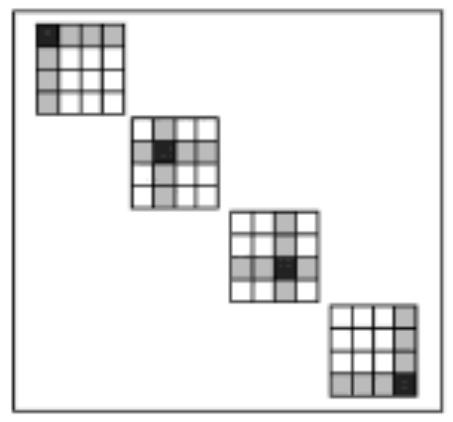
\includegraphics[scale=0.5]{FW_SEQ_TILED2.png}
  \end{center}
\end{minipage}
~\\\\\\
\indent Este algoritmo es hecho para que sea cache-oblivious, de manera que un bloque sea del tamano del cache. En efecto, para calcular cada bloque, solo necesita de cargar 1 bloque en etapa 1, 2 bloques en etapa 2, y 3 bloques en etapa 3.

\subsection{Floyd-Warshall paralelo, con una matriz cortada en bloques cuadrados}

\noindent Codigo de entrada : FW\_PAR\_TILED \\
Codigo de salida : FWPTI (Floyd-Warshall parallel tiled-implemented)\\

Es la version paralela del algoritmo anterior.

\subsection{Floyd-Warshall secuencial, con una matriz cortada en bloques cuadrados, con una disposicion adaptada de la memoria}

\noindent Codigo de entrada : FW\_SEQ\_TILED\_LAYOUT \\
Codigo de salida : FWSTB (Floyd-Warshall secuencial tiled-bloc implemented)

\begin{center}
  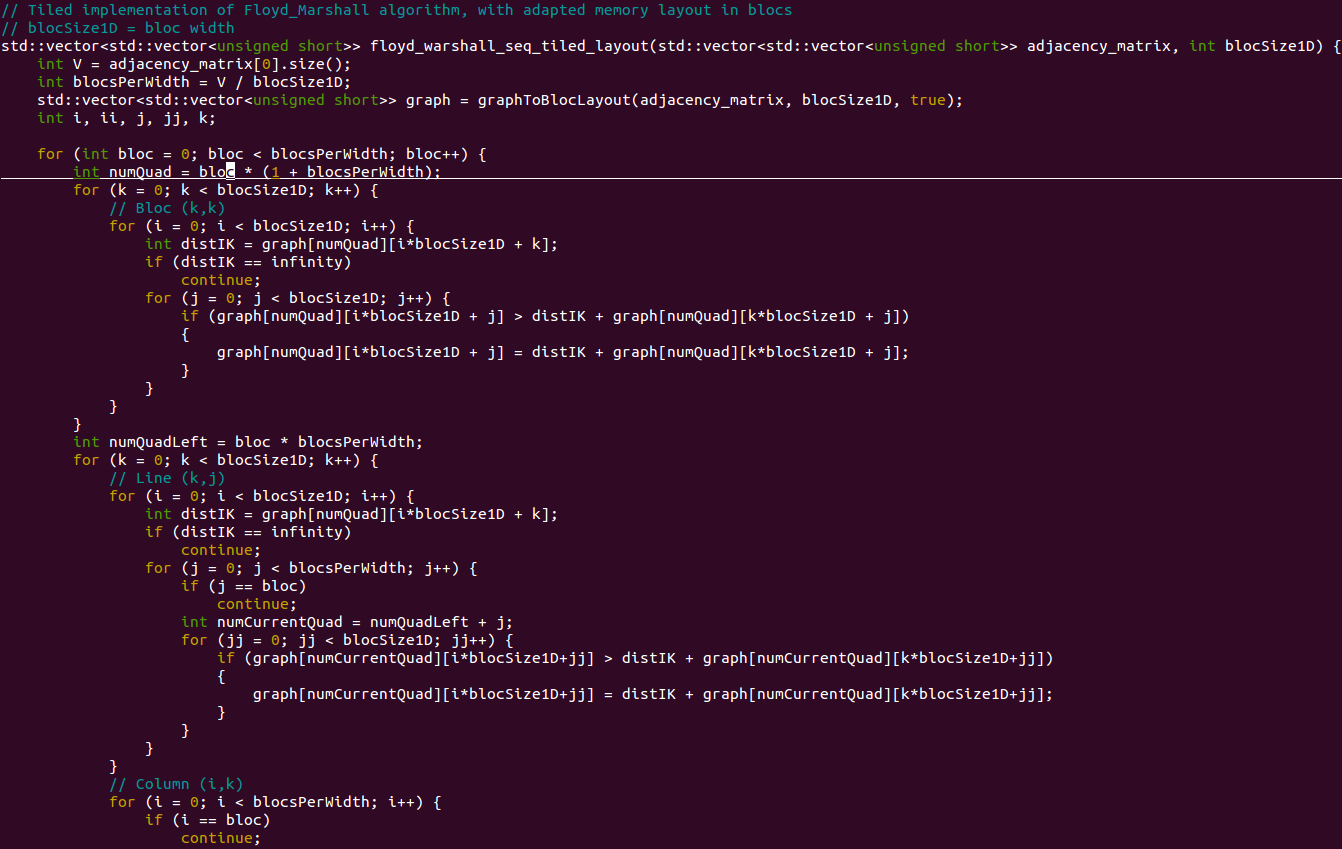
\includegraphics[scale=0.5]{FW_SEQ_TILED_LAYOUT.png}
\end{center}

Es lo mismo algoritmo que antes, pero con una dispocision adaptada de la memoria, en bloques. Es lo que la linea 3 del algoritmo hace.

Asi se reduce el numero de fallas de cache.

\subsection{Floyd-Warshall paralelo, con una matriz cortada en bloques cuadrados, con una disposicion adaptada de la memoria}

\noindent Codigo de entrada : FW\_PAR\_TILED\_LAYOUT \\
Codigo de salida : FWPTB (Floyd-Warshall parallel tiled-bloc implemented)\\

Es la version paralela del algoritmo anterior. Deberia estar el mejor algoritmo.

\subsection{Floyd-Warshall secuencial, con una matriz en una dimensión}

\noindent Codigo de entrada : FW\_SEQ\_1D \\
Codigo de salida : FWS1D

\begin{center}
  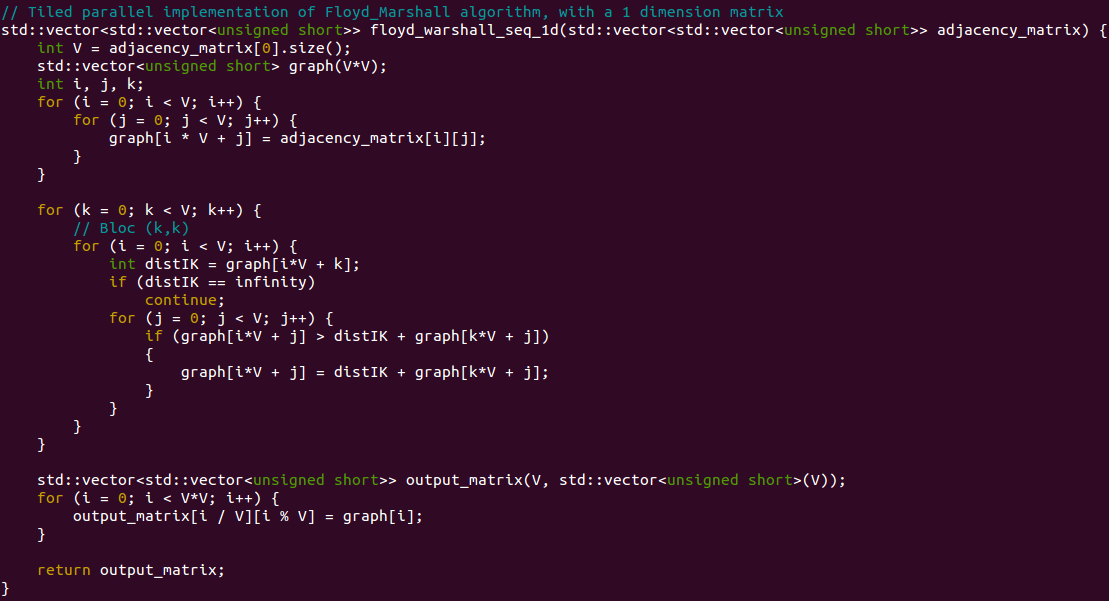
\includegraphics[scale=0.6]{FW_SEQ_1D.png}
\end{center}

Es el algoritmo basico (con las mejoracion de memorisacion y de saltar los infinitos), con una matriz en una dimensión.
Se puede ver como un caso especial del algoritmo de antes, cuando hay solo un bloque.

\subsection{Floyd-Warshall paralelo, con una matriz en una dimensión}

\noindent Codigo de entrada : FW\_PAR\_1D \\
Codigo de salida : FWP1D

\begin{figure}[H]
\begin{center}
  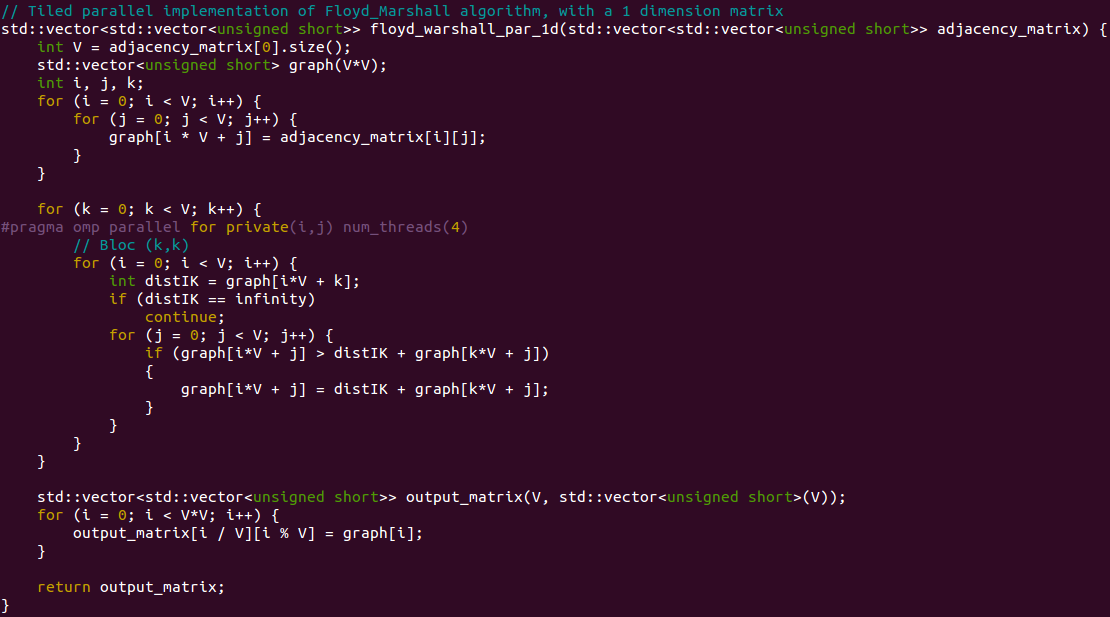
\includegraphics[scale=0.6]{FW_PAR_1D.png}
  \caption{Algoritmo de Floyd-Warshall paralelo con una matriz 1D}
\end{center}
\end{figure}

Es la version paralela del algoritmo anterior.

\subsection{Dijkstra secuencial}

\noindent Codigo de entrada : DIJK\_SEQ \\
Codigo de salida : DIJK\_SEQ

\begin{figure}[H]
\begin{center}
  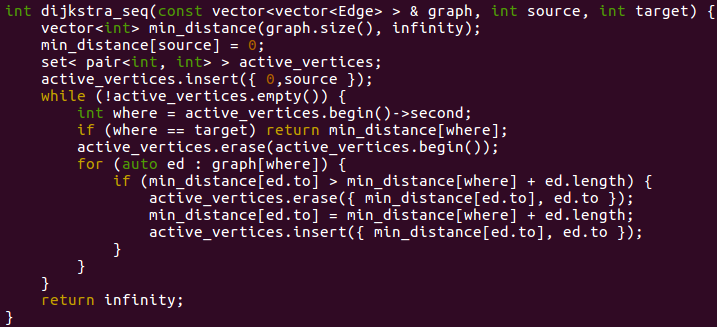
\includegraphics[scale=0.6]{DIJK.png}
  \caption{Algoritmo basico de Dijkstra}
\end{center}
\end{figure}

Es el algoritmo basico de Dijkstra, que a la diferencia de Floyd-Warshall calcula la distancia minima solo para ir de un vertice a un otro.

\section{Aseguramiento de exactitud de las salidas}
\subsection{''Realidad del terreno''}

Al principio, testé la exactitud de las salidas del algoritmo basicó. Como el codigo del algoritmo es bastante facil y se puede encontrar sobre el internet, solo testé sobre los grafos basicos.

El script Python \textbf{Verify\_Output.py} permite de verificar que las salidas para los grafos basicos estan los mismos que los que se encontran en la carpeta Ground\_Truth, que estan hecho de mano.

Tambien para verificarlos, el script \textbf{Graph\_Generator.py} permite de generar grafos como el de la figura 2. Functiona solamento para los grafos basicos.

\subsection{Script de comparación de la salidas}

Después de usar la opción -d del main (para escribir las salidas de los diferentes algoritmos en archivas), se puede comparar las salidas de cada algoritmo.

\begin{minipage}{0.35\linewidth}
El script al lado hace la diferencia entre las archivas, para ver si los algoritmos producen todos la misma salida.\\

Si todos los algoritmos producen la misma salida que el algoritmo basicó, consideramos que los algoritmos estan exactos, aunque puede haber diferentes casos límite, que no estan interesantes.
\end{minipage}\hfill
\begin{minipage}{0.65\linewidth}
  \begin{center}
    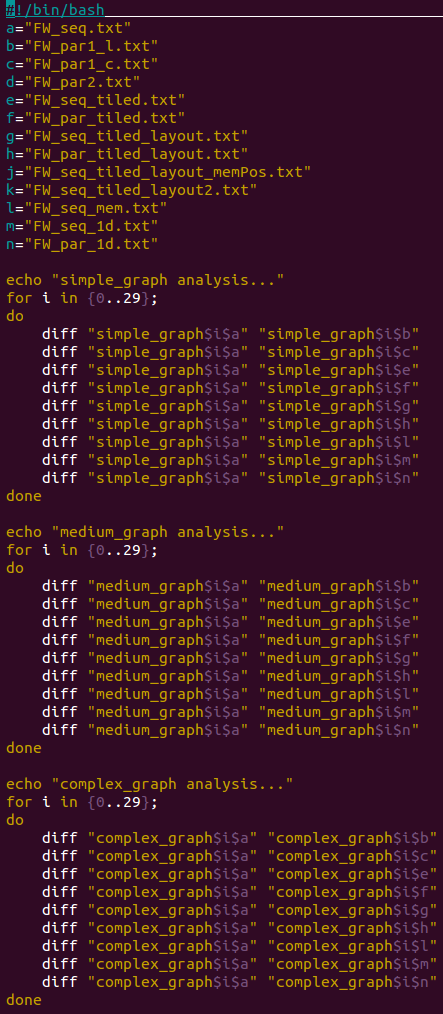
\includegraphics[scale=0.55]{diff_script.png}
  \end{center}
\end{minipage}

\section{Comparación de desempeño}

Los grafos simples solo se utilizaron para probar los algoritmos, vamos a utilizar los otros para comparar los desempenos.

La configuracion utilizada es :

\begin{itemize}
  \item Processor : Intel(R) Core(TM) i5-3210M CPU @ 2.50GHz
  \item 4 threads
  \item Tamano de cache : 3072 KB
  \item Compilador : gcc 6.2
  \item Optimizacion : O3
\end{itemize}

\subsection{Grafos medios}

\begin{center}
  \begin{tabular}{p{2cm} | p{4.5cm} | p{2cm} | p{3cm} | p{3cm}}
    \centering \textbf{Algoritmo} & \centering \textbf {Veces mejor que el algo basico} & \centering \textbf{Tiempo total} & \centering \textbf{Mejor caso} & \centering \textbf{Peor caso} \tabularnewline
    \hline
    FWSeq & & 6.41 & & \\
    \hline
    \hline
    FWSqM & 29 & 6.24 & 118\% mejor & 0\%, igual \\
    \hline
    FWSTB & 15 & 5.33 & 2308\% mejor & 68\% peor \\
    \hline
    FWSTI & 23 & 2.95 & 4433\% mejor & 64\% peor \\
    \hline
    FWP1C & 28 & 2.95 & 3640\% mejor & 38\% peor \\
    \hline
    FWP1L & 30 & 2.80 & 4084\% mejor & 16\% mejor \\
    \hline
    FWS1D & 23 & 2.66 & 3913\% mejor & 63\% peor \\
    \hline
    FWSMS & 30 & 2.48 & 17600\% mejor & 17\% mejor \\
    \hline
    FWPTB & 30 & 2.32 & 3379\% mejor & 6\% mejor \\
    \hline
    FWPTI & 29 & 1.39 & 5745\% mejor & 60\% peor \\
    \hline
    FWP1D & 30 & 1.25 & 6946\% mejor & 100\% mejor \\
    \hline
  \end{tabular}
\end{center}

\subsection{Grafos complejos}

\begin{center}
  \begin{tabular}{p{2cm} | p{4.5cm} | p{2cm} | p{3cm} | p{3cm}}
    \centering \textbf{Algoritmo} & \centering \textbf {Veces mejor que el algo basico} & \centering \textbf{Tiempo total} & \centering \textbf{Mejor caso} & \centering \textbf{Peor caso} \tabularnewline
    \hline
    FWSeq & & 94.24 & & \\
    \hline
    \hline
    FWSqM & 25 & 93.97 & 2\% mejor & 7\% peor \\
    \hline
    FWSTB & 16 & 74.94 & 4671\% mejor & 47\% peor \\
    \hline
    FWP1C & 30 & 60.23 & 747\% mejor & 1\% mejor \\
    \hline
    FWP1L & 30 & 49.36 & 3891\% mejor & 11\% mejor \\
    \hline
    FWSTI & 30 & 44.19 & 6010\% mejor & 12\% mejor \\
    \hline
    FWSMS & 30 & 38.79 & 11861\% mejor & 24\% mejor \\
    \hline
    FWS1D & 30 & 38.69 & 6952\% mejor & 24\% mejor \\
    \hline
    FWPTB & 30 & 28.76 & 6318\% mejor & 57\% mejor \\
    \hline
    FWPTI & 30 & 20.88 & 7547\% mejor & 100\% mejor \\
    \hline
    FWP1D & 30 & 17.73 & 11506\% mejor & 100\% mejor \\
    \hline
  \end{tabular}
\end{center}

\subsection{Grafos re complejos}

\begin{center}
  \begin{tabular}{p{2cm} | p{4.5cm} | p{2cm} | p{3cm} | p{3cm}}
    \centering \textbf{Algoritmo} & \centering \textbf {Veces mejor que el algo basico} & \centering \textbf{Tiempo total} & \centering \textbf{Mejor caso} & \centering \textbf{Peor caso} \tabularnewline
    \hline
    FWSeq & & 1007 & & \\
    \hline
    \hline
    FWSTB & 2 & 1535 & 263\% mejor & 54\% peor \\
    \hline
    FWP1C & 7 & 1243 & 33\% mejor & 37\% peor \\
    \hline
    FWSqM & 20 & 1016 & 3\% mejor & 8\% peor \\
    \hline
    FWP1L & 13 & 1006 & 107\% mejor & 30\% peor \\
    \hline
    FWSTI & 30 & 729 & 232\% mejor & 6\% mejor \\
    \hline
    FWSMS & 30 & 706 & 215\% mejor & 11\% mejor \\
    \hline
    FWS1D & 30 & 694 & 263\% mejor & 12\% mejor \\
    \hline
    FWPTB & 29 & 589 & 641\% mejor & 9\% mejor \\
    \hline
    FWPTI & 30 & 365 & 585\% mejor & 36\% mejor \\
    \hline
    FWP1D & 30 & 335 & 647\% mejor & 100\% mejor \\
    \hline
  \end{tabular}
\end{center}

\subsection{Analisis}

\indent Este parte es solamente relativa a mi maquina. Los resultados pueden ser muy diferentes sobre maquinas mas poderosas, por eso el manual del usario en parte 2 permite de hacer tests de desempeño sobre otras maquinas.

Podemos ver que el algoritmo paralelo con la matriz en una dimensión es el mejor. 

Es un caso especial del algoritmo en bloques, que teoricamente deberia estar mejor. Ademas el algoritmo FWPTI, que es el FWPTB sin cambiar la representacion en memoria de la matriz, tiene mejor desempeno. Eso es extrano porque normalmente el cambio de la representacion en memoria es hecho para reducir las fallas de cache, y con gprof se puede ver que las funciones para cambiar la representacion de la matriz no toman mucho tiempo, la diferencia no se puede explicar de ese manera.

Tambien podemos ver que el algoritmo basico con memorisacion tiene casi el mismo desempeno que el algoritmo basico. Eso se explica con el O3 de gcc 6.2. En efecto trabajé casi todo el tiempo con gcc 4.8.4 y el O3, y con eso este algoritmo fue mucho mejor en comparison con el algoritmo basico con gcc 4.8.4 O3.

Entonces se puede deducir que el O3 ahora es suficiente inteligente para hacer la memorisacion solo.

De otro lado, los resultados de mejor caso se pueden explicar con los saltos de las valores infinitas. Los 30 grafos fueron hecho de manera aleatoria, entonces si hay una proporcion muy importante de aristas infinitas, el algoritmo basico va a estar peor en comparison. Por eso aunque E no influye la complejidad, influye el desempeño.

Ademas,  el algoritmo FWP1L es mejor que el algoritmo FWP1C, porque las lineas de la matriz son localizadas en la memoria (aun con std::vector). Pero no estan buenos, porque estan peor que el algoritmo FWSMS mientras que usan las mismas metodas.

\section{Analisis comparativa de los algoritmos mas interesantes, sobre grafos de referencia}

En las tablas por debajo se pueden encontrar los tiempos de calcul de los algoritmos mas interesantes, expresados en segundos.

\subsection{Con O3}

\begin{center}
  \begin{tabular}{p{3.5cm} | p{1.6cm} | p{1.6cm} | p{1.8cm} | p{1.8cm} | p{1.8cm} | p{1.8cm}}
    \textbf{Algoritmo} &  \textbf{V = 400} &  \textbf{V = 800} &  \textbf{V = 1200} &  \textbf{V = 1600} &  \textbf{V = 2000} &  \textbf{V = 3200} \\
    \hline
    Basico & 0.062 & 0.40 & 1.32 & 3.15 & 6.12 & 24.36 \\
    \hline
    Basico con memorisacion & 0.059 & 0.40 & 1.31 & 3.16 & 6.11 & 24.38 \\
    \hline
    Basico con memorisacion y saltos de infinitas & 0.051 & 0.30 & 0.77 & 1.33 & 1.96 & 10.37 \\
    \hline
    secuencial 1d & 0.069 & 0.33 & 0.81 & 1.41 & 2.02 & 10.54 \\
    \hline
    Paralelo 1d 2 threads & 0.039 & 0.18 & 0.45 & 0.75 & 1.09 & 5.67 \\
    \hline
    Paralelo 1d 4 threads & 0.032 & 0.15 & 0.39 & 0.64 & 0.95 & 5.08 \\
    \hline
  \end{tabular}
\end{center}

\subsection{Sin O3}

\begin{center}
  \begin{tabular}{p{3.5cm} | p{1.6cm} | p{1.6cm} | p{1.8cm} | p{1.8cm} | p{1.8cm} | p{1.8cm}}
    \textbf{Algoritmo} &  \textbf{V = 400} &  \textbf{V = 800} &  \textbf{V = 1200} &  \textbf{V = 1600} &  \textbf{V = 2000} &  \textbf{V = 3200} \\
    \hline
    Basico & 1.03 & 8.08 & 27.1 & 64.29 & 125.9 & 514 \\
    \hline
    Basico con memorisacion & 0.73 & 5.76 & 19.28 & 45.65 & 89.1 & 352 \\
    \hline
    Basico con memorisacion y saltos de infinitas & 0.63 & 4.03 & 10.47 & 17.35 & 25.3 & 145 \\
    \hline
    Secuencial 1d & 0.42 & 2.64 & 6.86 & 11.37 & 16.6 & 94 \\
    \hline
    Paralelo 1d 2 threads & 0.40 & 1.57 & 4.13 & 6.93 & 11.73 & 56 \\
    \hline
    Paralelo 1d 4 threads & 0.23 & 1.46 & 3.75 & 6.25 & 9.91 & 52 \\
    \hline
  \end{tabular}
\end{center}

\section{Explicacion de los resultados}
\subsection{La importancia de la gestion del cache en linea}

En c++ la memoria es organizada en lineas, entonces es mucho mas rapido de examinar una tabla linea per linea que columna per columna. Se puede ver aqui por ejemplo :

\begin{center}
  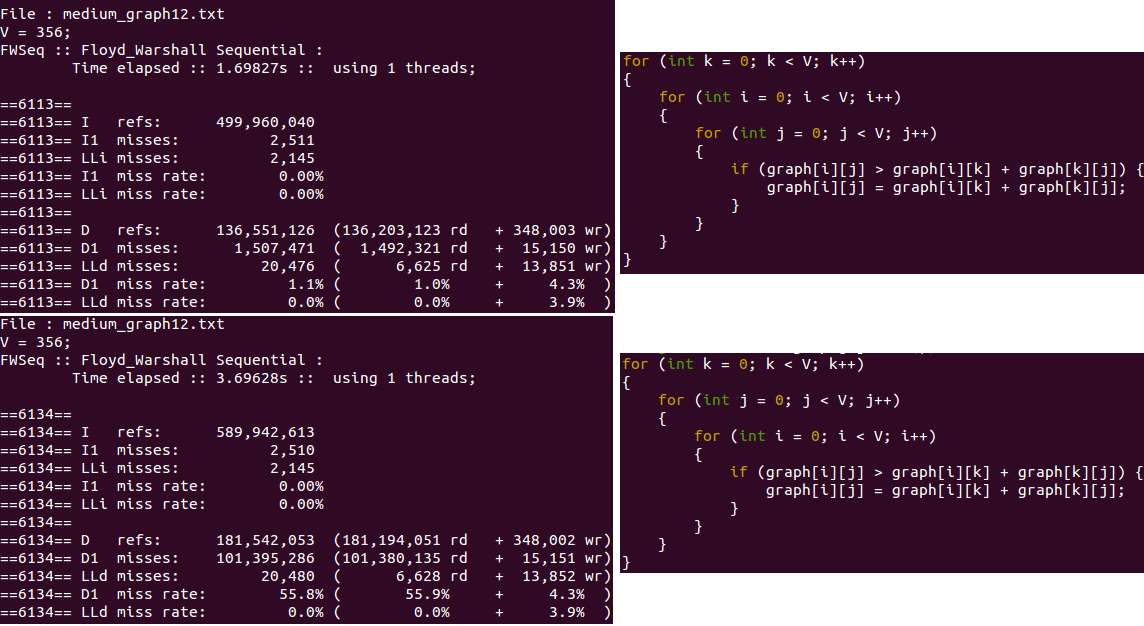
\includegraphics[scale=0.6]{Cache_Importance.png}
\end{center}

Para explicarlo, nos interemos a la ultima boucla for en cada caso.\\

En el primer caso, graph[i][k] es una constante en la boucla, solamente graph[i][j] y graph[k][j] depienden de la variable de la boucla. Por eso, para cargar todas las valores de la boucla, solo hay que cargra las lineas i y k de la matriz.\\

En el secondo caso, son graph[i][j] y graph[i][k] que depienden de la variable de la boucla. Pero por cada valor de i, hay que cargar en la memoria una nueva linea de la matriz.

\noindent Eso genera muchas fallas de cache, y explica porque el segundo caso es mucho mas lento que el primero.

\subsection{La importancia de la ubicación espacial en la memoria}

Este parte sirve a explicar porque el algoritmo con la matriz en una dimensión es el mejor.

Como el tamaño de la matriz de distancias es conocido que durante la ejecución, las tablas estan dinamicas.

Por eso usé vectores de vectores. Functionan como una tabla 2D en C, con punteros de punteros.

Pero cuando la matriz no esta en una dimensión, la localidad espacial en la memoria se pierde, porque cada linea puede ser lejos de una linea consecutiva.

\section{Possibilidades de mejoracion}

La primera cosa a hacer es de testear los desempeños sobre una maquina mas poderosa. El mejor algoritmo deberia ser el FWPTB, con un tamaño de bloque que esta del tamaño del cache. El script Python \textbf{generate\_blocsize\_analysis.py} puede testear diferentes tamaños de bloques. Se llama desde la carpeta primaria.

De otra parte, es posible de implementar el algoritmo de Floyd-Warshall de manera recursiva, con el Z-Morton layout.

\section{Bibliografia}

Tutorial OpenMP :

https://computing.llnl.gov/tutorials/openMP/\\

\noindent Algoritmo de Floyd-Warshall :

https://www.cs.usfca.edu/galles/visualization/Floyd.html

http://www.mcs.anl.gov/itf/dbpp/text/node35.html

http://www.infor.uva.es/diego/docs/ortega13b.pdf

http://www.cse.buffalo.edu/faculty/miller/Courses/CSE633/Muthuraman-Spring-2014-CSE633.pdf

http://courses.csail.mit.edu/6.884/spring10/projects/kelleyk-neboat-slides.pdf

http://citeseerx.ist.psu.edu/viewdoc/download?doi=10.1.1.40.5378\&rep=rep1\&type=pdf

https://prezi.com/z9eiteeaqxmh/parallel-approach-to-floyd-warshall-algorithm/

https://people.cs.kuleuven.be/george.karachalias/papers/floyd-warshall.pdf

http://moais.imag.fr/membres/marc.tchiboukdjian/pub/thesis.pdf

http://escholarship.org/uc/item/9v89p5wv\#page-10

http://repository.upenn.edu/cgi/viewcontent.cgi?article=1213\&context=hms

https://www.google.com.ar/url?sa=t\&rct=j\&q=\&esrc=s\&source=web\&cd=1\&ved=0ahUKEwjUpeKBxO\_PAhWIH5AKHb2zBLcQFggcMAA\&url=http\%3A\%2F\%2Fwww.cs.technion.ac.il\%2Fitai\%2FCourses\%2FCache\%2FPresentations\%2Foptimizing-gr-algs.ppt\&usg=AFQjCNEidlujtiLvwSzdGqEQ56XNeDyrKA\&cad=rja\\


\noindent Z-Morton order :

https://en.wikipedia.org/wiki/Z-order\_curve\\


\noindent Cache defaults :

http://valgrind.org/docs/manual/cg-manual.html

http://igoro.com/archive/gallery-of-processor-cache-effects/


\end{document}
